\chapter{Benutzerschnittstelle des Chatbots}
\label{sec:Benutzerschnittstelle}

Da eine Konsole nicht als benutzerfreundlich einzustufen ist, brauchten wir noch eine Benutzerschnittstelle. ChatScript bietet hier auch mehrere Möglichkeiten an, unter anderem gibt es eine serverbasierte Version, die von vorneherein mitgeliefert wird (s. ChatScript - ClientServer - Manual in \citet{chatscript2019}). Allerdings sind wir beim Einrichten auf mehrere Probleme gestoßen, auf die in \ref{sec:Probleme} näher eingegangen wird. Aufgrund dieser Probleme war es leider nicht möglich, die Benutzerschnittstelle mit dem Chatbot im Ganzen zu verwenden, weshalb im Folgenden nur kurz und der Vollständigkeit halber auf die GUI eingegangen werden soll.\\
Die vorgegebene serverbasierte Version war vorteilhaft, da sie zum einen die potentielle spätere Einbindung in den Uni-Shop auf der Webseite der Universtiät Trier ermöglicht und zum anderen kaum Aufwand unsererseits für die Konstruktion einer eigenen GUI nötig war. Lediglich Stylesheet-Befehle wurden eingefügt, um das Design unseren Bedürfnissen anzupassen.\\
Abbildung \ref{ScreenshotGUI} zeigt einen Screenshot der Benutzerschnittstelle. Die Darstellung betreffend haben wir den Stil der Webseite der Universität nachgebildet, um die Zugehörigkeit zu betonen. So befindet sich in der linken oberen Ecke das Universitätslogo und rechts daneben auf dunkelblauen Grund in weißer Schrift die Überschrift des Chatbots. Die Kommentare Augustas und die des Kunden erscheinen in Sprechblasen. Augustas sind blassblau, da blau die dominantere Farbe im Farbschema der Universität ist. Das Gesagte des Kunden ist blassgrün, da auch grün mit der Institution assoziiert wird.\\


\begin{figure}
\begin{center}
{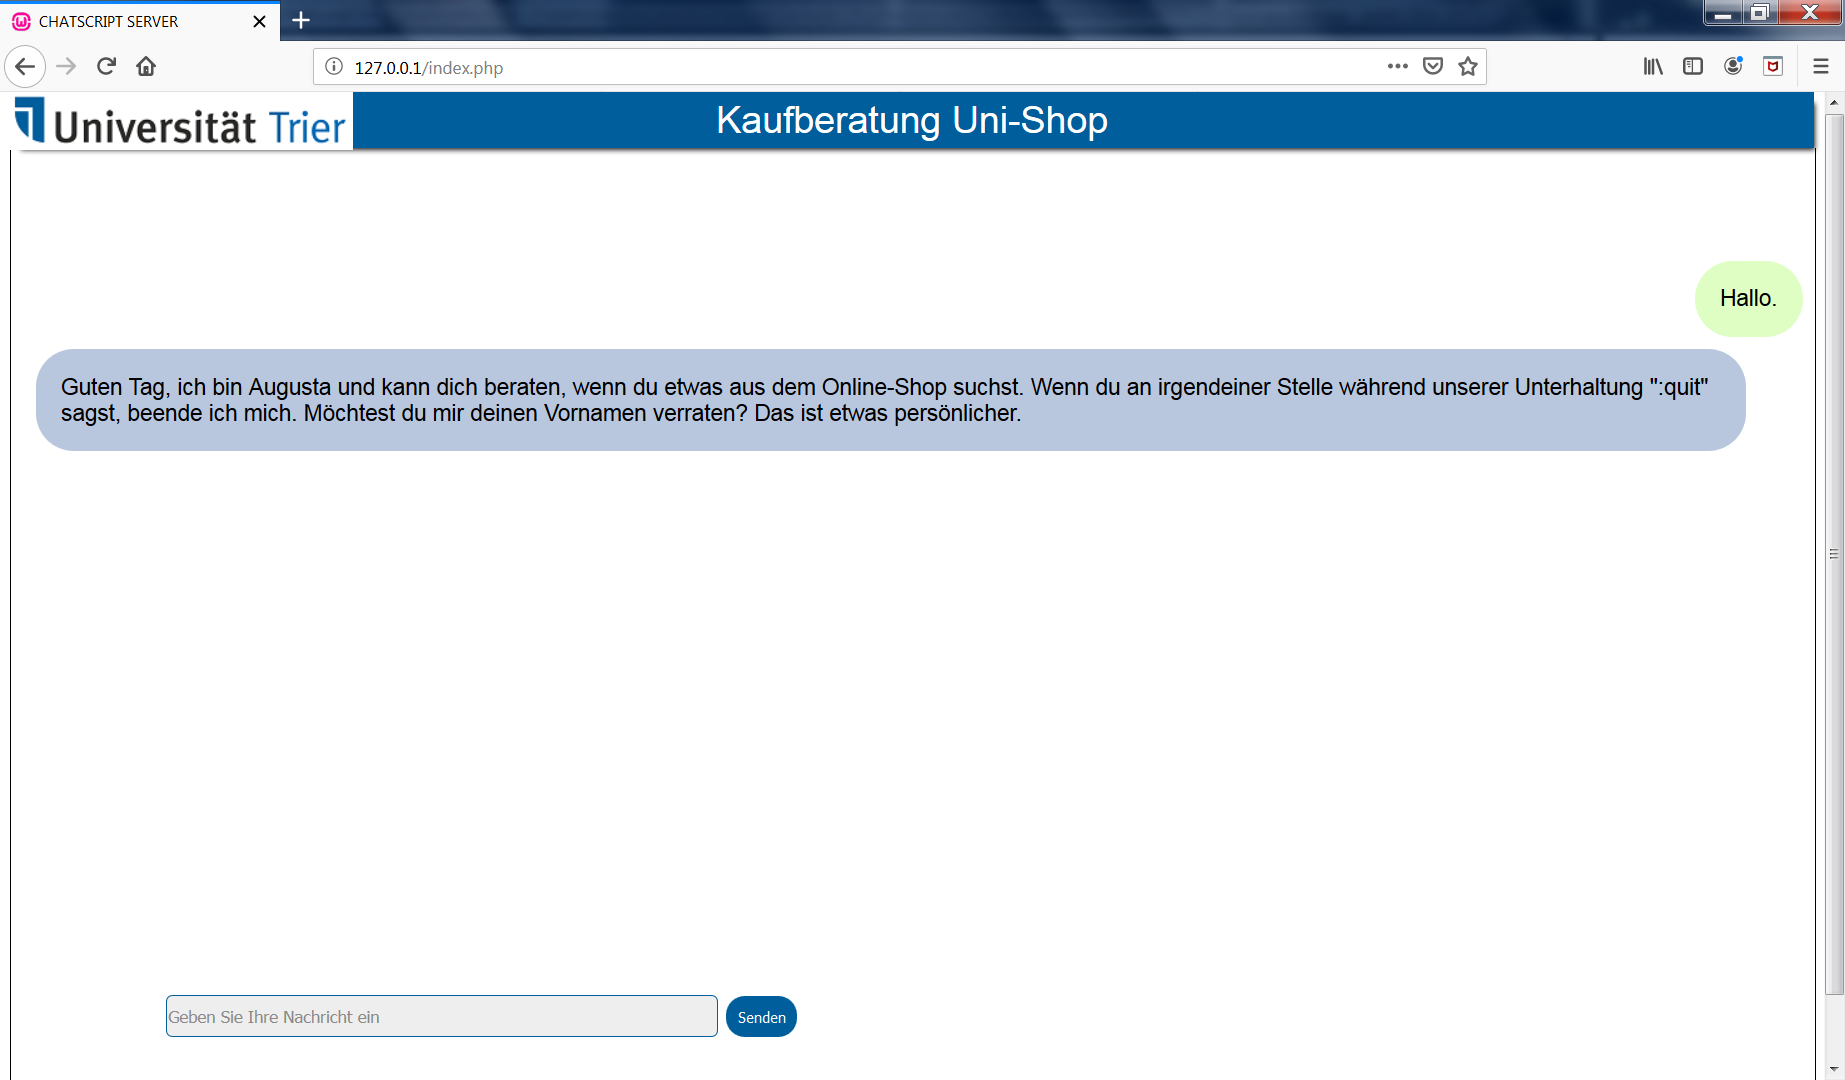
\includegraphics[width=8cm]{BILDER/gui.png}}
\end{center}
	\caption{Screenshot der Benutzerschnittstelle}
	\label{ScreenshotGUI}
\end{figure}
